\documentclass[../zhang_thesis.tex]{subfiles}
\begin{document}

\chapter{Introduction}

Batteries, particularly rechargeable ones, are used extensively in daily life. They provide the energy for such electrical systems as communication, automotive, and renewable power systems. In order to design for and operate these systems, an accurate battery model and a means of simulating the model efficiently is needed. For example, modern battery charge and health management schemes use high-fidelity battery models to track the state of charge (SOC) and state of
health (SOH); this information is then used to predict and optimize the runtime of the battery. However, widely-used chemical batteries have nonlinear capacitive effects, which require the use of a nonlinear filter for accurate prediction of its states in the presence of noise. This thesis explores one possible solutions to this problem by choosing an appropriate battery model and testing the accuracy of various nonlinear filters in determining the SOC through simulation.

%%%%%%%%%%%%%%%%%%%%%%%%%%%%%%%%%%%%%%%%%%%%%%%%%%%%%%%%%%%%%%%

\section{Electrical Characteristics of Rechargeable Batteries}

A high-fidelity battery model has to accurately reproduce the various characteristics of a battery. Most models keep track of the total capacity and SOC in order to predict remaining runtime. More accurate models include nonlinear effects, such as the rate-capacity effect and the recovery effect, along with self-discharge and the effects of ambient temperature. The dynamic electrical attributes, such as the current-voltage (i-v) characteristics and transient responses, can also be
modeled. The remainder of this section defines these characteristics.

The capacity of a battery is the amount of electric charge it can store, measured in the SI unit Ampere-hours (Ah). Commonly, for rechargeable battery specifications, the subunit milliampere-hour (mAh) is used. Related is the available capacity, which is the amount of charge available for use. Due to the electrochemical nature of batteries, a battery's available capacity decreases as the rate of discharge increases, known as the rate-capacity effect. Therefore, the capacity for a
battery is typically stated for a given discharge rate.  Related to this is the recovery effect, so called because when a battery is allowed to rest during an idle period, the battery ``recovers'' available capacity previously lost during discharge due to the rate-capacity effect. Thus, a battery discharged at a high rate until seemingly fully discharged, when allowed to rest, regains a portion of its lost capacity.

Both the rate-capacity effect and the recovery effect can be explained by the electrochemical nature of the battery. During discharge, the concentration of the active material around the electrode is depleted, and the active materials in the depletion region move towards the electrode to reduce the concentration gradient~\cite{chiasserini99}. Because the speed at which the concentration gradient is equalized is limited, the faster the rate of discharge, the less the active material is
replenished, resulting in a decrease in the available capacity. Likewise, when the battery is allowed to rest, the active material gradient has additional time to equalize, and the available capacity is increased.

Closely related to the capacity is the SOC. This thesis defines it as the ratio between the remaining capacity and the maximum capacity, with both capacities measured using the amount of active material within the battery. This definition then denotes the proportion of remaining chemical energy rather the available energy and is unaffected by the rate-capacity and recovery effects. Note that a fully charged battery has an SOC of unity and a fully discharged battery has an SOC of
zero, regardless of the available capacity. Additionally, it is convenient to establish the relationship between the SOC of the battery and its open-circuit voltage $V_{OC}$, which is useful for simulation of the i-v characteristics and transient responses. $V_\text{OC}$ can be thought as the limit of the measured battery voltage after recovery.

Other more minor effects that are usually incorporated into models are self-discharge, the effect of ambient temperature, and aging. Self-discharge refers to an idle battery decreasing its SOC over time due to internal chemical reactions. It is dependent on the type of battery, SOC, ambient temperatures, and other factors. The ambient temperature has effects on the internal resistance of the battery and the self-discharge rate. Commonly, the battery is designed to operate with a narrow range of temperatures. Below the operating temperature range, the internal resistance increases, decreasing the capacity. Above the operating range, the internal resistance decreases, not only increasing the capacity but also the self-discharge rate; thus, the actual capacity is lowered due to the increased self-discharge. Aging refers to the decrease in battery performance measures, such as capacity, self-discharge, and internal resistance, over time due to unwanted chemical reactions. In practice, aging is indicated by the SOH, defined as the ratio between the current maximum capacity and that of a new battery. The SOH threshold at which the battery performance is considered too degraded varies by application.

%This thesis studied the prediction of the SOC of a battery using noisy measurements of its current and voltage. To do so accurately for a general load, incorporation of the rate-capacity and recovery effects as well as the transient i-v characteristics is desirable. Furthermore, it is useful to have a model easily tunable for different battery types. The following section reviews the characteristics of different battery models and chooses the one most suitable for the purposes of this study.

%%%%%%%%%%%%%%%%%%%%%%%%%%%%%%%%%%%%%%%%%%%%%%%%%%%%%%%%%%%%%%%

\section{Battery Models}

This thesis studied the predition of the SOC of a battery given knowledge of the resistive load on the battery as well as noisy measurements of the voltage across its terminals. In order to do so for a general load profile, incorporation of the rate-capacity and recovery effects as well as the transient i-v characteristics is desirable. Furthermore it is useful to have a model easily tunable for different battery types. This section reviews the characteristics of major types of
battery models. Battery models can be divided into five categories, namely electrochemical, computational intelligence, analytical, stochastic, and electrical-circuit. The remainder of this section reviews each type and determines the most suitable battery model for this study.

\subsection{Electrochemical}

Electrochemical models are describe the chemical processes that place in the battery in great detail. These are generally the most accurate, but they require in-depth knowledge of the chemical processes to create and impose large computational costs~\cite{jongerden09}. One of the most widely known electrochemical models was developed by Doyle, Fuller, and Newman for lithium and lithium-ion batteries using noninvasive voltage-current cycling
experiments~\cite{doyle93,fuller94,fuller94b}. It consists of six coupled, nonlinear differential equatons that capture lithium diffusion dynamics and charge transfer kinetics. The model is able to predict i-v response and provides a design guide for thermodynamics, kinetics, and transport across electrodes. A implementation of their model in Fortran, called Dualfoil, is available for free online.\footfullcite{newman98} The program needs more than 60 parameters along with the load profile
in order to compute the battery properties. Setting the parameters requires detailed knowledge of the battery, but the result of the program is highly accurate. Other battery models are often compared to it rather than to experimental results.

\subsection{Computational Intelligence}

Computational intelligence is a brance of computer science interested in problems that require the intelligence of humans and animals to solve. One of the earliest definitions by Bezdek states that computational intelligent systems use pattern recognition on low-level, numerical data and do not use knowledge as with artificial intelligence~\cite{bezdek92,bezdek94}. Methods such as neural networks, fuzzy systems, and evolutionary computation are commonly classified as computational
intelligence. Battery models using such methods as neural networks~\cite{ogorman98,capizzi11}, support vector machines~\cite{wang06}, and hybrid neural-fuzzy models~\cite{shen02} have been studied. These models learn the nonlinear relationships between battery properties, such as SOC, current, voltage, and temperature, through a computationally costly training process. However, once trained, they incur a much lower cost and can achieve comparable accuracy to electrochemical
models.

\subsection{Analytical}

Analytical models are simplified electrochemical models that trade off accuracy for simplicity. One of the simplest such models is Peukert's law for lead-acid batteries, which states that for a one-ampere discharge rate~\cite{doerffel06}
\begin{equation}
C_p = I^k t,
\end{equation}
where $C_p$ is the capacity at a one-ampere discharge rate in Ah, $I$ is the discharge current in A, $t$ is the time to discharge the battery in hours, and $k\ge 1$ is the dimensionless Peukert constant, typically between 1.1 and 1.3 for a lead-acid battery. The constant $k$ only equals unity for an ideal accumulator, so for real batteries, $k$ is always greater than unity. Thus, for a given increase in the discharge current, the discharge time decreases by a proportionally greater
amount. Therefore, the effective, or available, capacity $C\times t$ is reduced. Peukert's law can be extended to some other battery chemistries, such as lithium-ion. Note that Peukert's law only models the rate-capacity effect and not the recovery effect. More complicated models, such as the kinetic battery model and the diffusion model, are able to describe both effects.

The kinetic battery model (KiBaM), initially created for large lead-acid batteries, describes the battery as a kinetic process, using two charge wells for the bound and available charges connected by a valve whose flow rate is proportional to the height difference between the wells~\cite{manwell93}. The change of charge in the wells is given by
\begin{equation}
    \begin{cases}
        \dfrac{dy_1}{dt} = -I + k \left( h_2 - h_1 \right) \\
        \dfrac{dy_2}{dt} = -k \left( h_2 - h_1 \right),
    \end{cases}
    \label{eq:kibam}
\end{equation}
where $y_1,y_2$ are the charges, $h_1,h_2$ are the heights of the wells, the parameter $k$ controls the rate of charge flow between the wells, and $I$ is the applied load. The flow rate of the valve should be lower than the typical discharge rate of the battery. During discharge from the available-charge well, the bound charges flow through the valve to equalize the heights of the two wells. It can be seen that for slower discharge rates, more charge flows through the valve and the effective
capacity increases. Likewise, during idle periods for the battery, the available charge increases.

Related to the KiBaM is the diffusion model, which describes the movement of the ions in the electrolyte of a lithium-ion battery~\cite{rakhmatov01}. Like in the kinetic battery model, the difference in the concentration of adjacent ions along the length of the battery determines the diffusion rate of the ions. The available charges are those ions directly touching the electrode of the battery. It can be seen that the KiBaM is a first-order approximation of the diffusion
model~\cite{jongerden09}, since the individual ions in the diffusion model are replaced by two charge wells in the KiBaM.

\subsection{Stochastic}

Stochastic models describe the discharging and the recovery effect as stochastic processes. The first models were developed by Chiasserini and Rao and based on discrete-time Markov chains~\cite{chiasserini99b}. They studied two models of a battery in a communication device that transmitted packets. The simpler model described the battery as a discrete-time Markov chain with $N+1$ states, numbered from $0$ to $N$ and corresponding to the number of charge units available in the battery.
Transmitting one packet requires one charge unit of energy. Thus, in continuous transmission, $N$ packets can be sent. At every time step, a charge unit is either consumed with probability $a_1=q$ or recovered with probability $a_0=1-q$. The battery is considered empty when the $0$ state is reached or when a theoretical maximum of $T$ charge units have been consumed. The second model is an extension of the first, allowing for more than one charge unit to be consumed in a time step, modeling
more bursty usage. Additionally, the battery has a non-zero probability of staying in the same charge state, indicating no consumption or recovery during a time step. Chiasserini and Rao extended their model further in following papers by adding state and phase dependence~\cite{chiasserini99,chiasserini01,chiasserini01b}. The state number is the number of charge units, and the phase number is the number of consumed charge units. Having fewer charge units decreases the probability of
recovery, while having more consumed charge units increases the probability of recover. Using these models, one can model different loads by setting the transitions probabilities. However, the order of the transitions is uncontrollable, so it is impossible to model fixed load patterns and compute their impact on battery life.

Chiasserini and Rao mainly investigated the gain $G$ in transmitted packets using a pulsed discharge relative to using a constant discharge, defined as $G=m/N$, where $m$ is the mean number of transmitted packets. The gain increases when the load decreases, due to an increase in the recovery probability. Additionally, the gain increases for lower discharge demand rates and higher current densities. These load profiles result in discharge currents close to the specified limits of the battery, causing the
available capacity to decrease overly quickly. Therefore, the recovery effect is especially strong for these cases during pulsed discharge, greatly increasing the gain. Chiasserini and Rao compared the computation of the gain parameter for different current densities and demand rates using the stochastic model to that of the electrochemical model of Doyle et al. They found an average deviation of 1\% and a maximum deviation of 4\%. This shows that the stochastic model accurately describes battery behavior during pulsed discharge. However, this model is only able to compute relative lifetimes.

In 2005, Rao et al.~\cite{rao05} proposed a stochastic battery model based on the Kinetic Battery Model (KiBaM) of Manwell and McGowan. This stochastic KiBaM was for a nickel-metal hydride (NiMH) battery. The differential equations governing the original KiBaM were modified to include an extra factor $h_2$ governing the flow of charge between the wells. This changes \autoref{eq:kibam} into
\begin{equation}
    \begin{cases}
        \dfrac{dy_1}{dt} = -I + k_s h_2 \left( h_2 - h_1 \right) \\
        \dfrac{dy_2}{dt} = -k_s h_2 \left( h_2 - h_1 \right),
    \end{cases}
\end{equation}
This change causes the recovery effect to weaken as the remaining charge decreases. The stochastic model was also modified to allow the possibility of no recovery during idle periods. The stochastic KiBaM describes the battery using a discrete-time, transient Markov process. The states are labeled with the parameters $(i,j,t)$, with $i$ and $j$ representing the discrete charge levels of the available and bound charge wells and $t$ representing the length of the current idle period.
Like the stochastic model of Chiasserini and Rao, it is impossible to fully model a real-life discharge pattern using the stochastic KiBaM. Rao et al.\ compared the results of their model with experimental results using an AAA NiMH battery. Two sets of experiments were conducted, the first with varying frequency of the load and a 50\% duty cycle and the second with varying off-time and a constant on-time. Their model accurately predicted the lifetime and delivered charge from the
battery, with a maximum error of 2.65\%.

\subsection{Electrical-Circuit}

Electrical-circuit models for batteries developed from the discovery of capacitative effects at the electrode-electrolyte interface. Helmholtz first proposed the existence of a double layer of charge at the interface in 1879. In 1899, Warburg proposed a series resistance and capacitance circuit model with an infinitely low current density. The Warburg capacitance $C_W$ named after him varies inversely with the square root of the frequency~\cite{geddes97}. In 1947, Randles proposed a model
consisting of a double-layer polarization capacitance $C_p$ in parallel with the series combination of a resistor $R$ and a capacitance $C$~\cite{randles47}. In 1994, Kovacs improved Randles circuit with the addition of Warburg impedence $Z_W$ replacing the capacitance $C$ and the solution resistance $R_s$ in series with the original Randles circuit~\cite{kovacs95}. In addition, he renamed $C_p$ to the double layer capacitance $C_{dl}$ and $R$ to the charge-transfer resistance
$R_{ct}$. These proposals came from a desire to represnt impedance spectra created using electrochemical impedance spectroscopy (EIS). The various elements in the models represent the different processes within a battery, which have different time constants. While these attempts model the impedance and, thus, account for the nonlinear rate-capacity and recovery effects, they do not consider the capacity and self-discharge of the battery.

%\begin{figure}[htb]
%    \centering
%    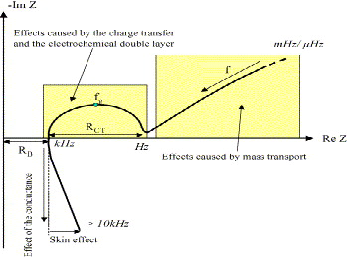
\includegraphics[width=0.8\textwidth]{nyquist_plot_batt}
%    \caption{Illustrative Nyquist plot of a battery~\cite{jossen06}. \emph{[Quite low quality from screen capture of article preview. I can recapture for better quality or recreate it.]}}
%    \label{fig:nyquist_plot_batt}
%\end{figure}

%\begin{figure}[htb]
%    \centering
%    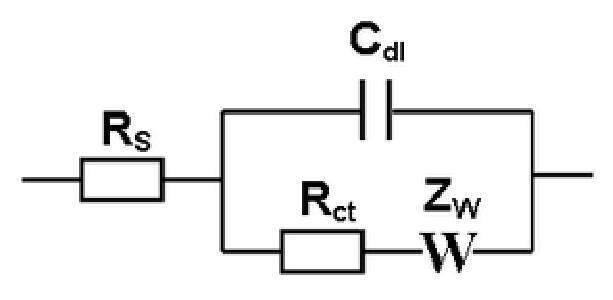
\includegraphics[width=0.6\textwidth]{randles_circuit}
%    \caption{Randles' equivalent circuit.}
%    \label{fig:randles_circuit}
%\end{figure}

In 1993, Hageman created simplified electrical-circuit models using PSpice for nickel-cadmium (NiCd), lead-acid, and alkaline batteries~\cite{hageman93}. The circuits shared the common elements of
\begin{enumerate*}[label=\emph{\roman*})]
\item a capacitor that represents the battery capacity,
\item a discharge rate normalizer that determines the additional capacity loss at high discharge rates,
\item a circuit that discharges the battery,
\item a lookup table of battery voltage versus SOC, and
\item a resistor that represents the battery's internal resistance~\cite{hageman93,hageman97}.
\end{enumerate*}
In addition, battery models for NiCd batteries simulated the thermal effects under high discharge rates. The main lookup table is formed by discharging a battery at a low rate at a constant current (20 to 200 hours). At high discharge rates, the discharge rate normalizer reduces the battery voltage below the value from looking up the SOC in the table. This normalizer is implemented using additional lookup tables. These circuit models are much simpler than electrochemical models, but they
are also less accurate with an approximate error of 10\%. Furthermore, creation of the lookup tables requires considerable data. These circuit-based models are mainly concerned with modeling the remaining discharge time and are referred to as runtime-based models.

In 2006, Chen and Rinc\'on-Mora proposed a combination of a runtime-based model and a impedance-based model consisting of a series resistor and two parallel resistor-capacitor networks~\cite{chen06}. The elements of the impedance part of the model had parameters that depended on the SOC. Additionally, the runtime model included a resistance that modeled the self-discharge rate. Their proposed model has the advantage of accurate prediction of the SOC using the runtime-based portion while also modeling
nonlinear transient effects, such as the rate-capacity and recover effects, with the impedance-based portion. Furthermore, the battery data can be collected using EIS measurements, which requires neither detailed knowledge of the battery chemistry nor lengthy, low-rate discharge experiments.

\subsection{Evaluation}

Of the model types, only some are fit for use with filtering algorithms. The computational-intelligence and stochastic models do not model the dyanmics of the battery system, so they cannot be used. The electrochemical models, the related analytical models, and the electrical-circuit models describe the system dynamics and the nonlinear rate-capacity and recovery effects. However, only the electrical-circuit model has the advantage of modeling the internal impedance of the battery,
which is useful in the design of battery systems. Of the electrical-circuit models, the proposal by Chen and Rinc\'on-Mora is best suited for the purposes of this thesis since it is the only one discussed by this paper that describes both the capacity and the transient effects. Therefore, their proposal is used for the simulation of the battery and comparing the performance of different filters.

%%%%%%%%%%%%%%%%%%%%%%%%%%%%%%%%%%%%%%%%%%%%%%%%%%%%%%%%%%%%%%%

\section{Nonlinear Filtering Methods}

Filtering refers to the methodology for estimating the state of a time-varying system that is indirectly observed through noisy measurements. Specifically, the current state is estimated from the current and previous measurements. The state of a system is a group of dynamic variables that evolve through time, and its evolution through time is governed by a dynamic system, perturbed by process noise. The measurements are functions of the state and measurement noise. A battery can be modeled as a
time-varying system, with state variables that describe such states as the SOC and the SOH. The measurements are typically the voltage and the current. Note that this thesis uses a resistive load instead of the current, because this is more realistic from a usage standpoint. Additionally, the SOH is not considered by this thesis. The dynamic system for the battery is described in more detail in the following chapter.

For linear systems, the optimal filtering solution with respect to the minimum mean squared error (MMSE) is given by the least squares solution, meaning the optimal least squares solution equals the posterior mean. A closed form solution to the discrete-time linearing filtering problem is given by the Kalman filter~\cite{kalman60}, which is a linear MMSSE (LMMSE) filter. Under the assumption that the noises are Gaussian, the posterior distribution is also Gaussian and numerical
approximations are unnecessary. The Kalman filter has a prediction phase and an update phase. The prediction phase estimates the current state using the state estimate from the previous time step. The update phase refines the state estimate using the current measurement.

For nonlinear systems, optimal filtering solutions are generally intractable, so various numerical approximation methods have been developed, mainly classified in three groups: function approximation, moment approximation, and stochastic model approximation~\cite{li04}. Function approximation techniques approximate the nonlinear dynamic and measurement processes, commonly using the Taylor series expansion. A moment approximation technique uses a representative
set of sample points and calculates integrals as weighted averages. Stochastic model approximation simplifies the original nonlinear stochastic system to a linear system so that linear filtering results are applicable.

Note that the choice of discretization method tends to depend on the filter, especially for highly nonlinear systems. Therefore, the simulations used a continuous-discrete (mixed) time system, with the form
\begin{align}
    \mathbf{\dot{x}}(t) &= \vf(\mathbf{x}(t),\mathbf{u}(t),\mathbf{w}(t)) \label{eq:gen_ct_f} \\
    \mathbf{z}_k &= \vh(\mathbf{x}(t_k),\mathbf{u}(t_k),\mathbf{v}(t_k)),
\end{align}
where $\vx$, $\vu$, $\mathbf{z}$, $\mathbf{w}$, and $\mathbf{v}$ are the vectors of the states, the inputs, the measurements, the process noises, and the measurement noises, respectively. For simplicity of simulation, the input $\mathbf{u}(t)$ is assumed to be constant over each time step so that $\mathbf{u}(t)=\mathbf{u}(t_k)$ for $t_k\le t < t_{k+1}$. For the prediction phase, the continuous-time dynamics were solved numerically, with each filter using different approximation
techniques. The state error covariances are also approximated numerically. Then, the updates were performed based on the update of the linear Kalman filter.

Furthermore, note that the system is extremely stiff for some inputs $\mathbf{u}$, which can be seen from the stiffness ratio based on the ratio of the largest eigenvalue of $F$ to its smallest eigenvalue, where $F$ is the jacobian of the dynamics $\vf(\mathbf{x},\mathbf{u})$; when the stiffness ratio is much greater than unity, the system is stiff~\cite{lambert91,brugnano11}. From EIS studies of batteries, the major chemical processes have widely differing time constants; low frequency
mass transport effects like diffusion are on the order of $10^{-6}$ to $10^0$ Hz, middle frequency effects caused by charge transfer and the electrochemical double layer are on the order of $10^0$ to $10^3$ Hz, and the high frequency conductance and skin effects are on the order of $10^3$ to $10^4$ Hz~\cite{jossen06}. Therefore, the approximate stiffness ratio is $10^{10} \gg 1$, and the system is stiff. As a result of the stiffness, any numerical integration method needs to be A-stable,
i.e.\ the method converges for all systems whose eigenvalues have negative real parts. For example, simulation results show that the fourth-order Runge-Kutta method diverges even at step sizes $<10^{-2}$ seconds.

S\"arkk\"a and Solin state that a linearized discretion approach, in which the continuous-time system is first discretized and then approximated as Gaussian, tends to work better than a discretized linearization approach, in which the system is first approximated as a Gaussian process and then discretized~\cite{sarkka12}. This thesis follows this guideline and performs the prediction using linearized approximations of a discretization of the continuous-time dynamics. The specifics of the
linearized discretion approach for each filter along with their general implementation are discussed in the remainder of this chapter.

\subsection{Function Approximation}

%The Taylor series expansion for a function $f(\mathbf{x},t)$ at $\hat{\mathbf{x}}$ is given by
%\begin{equation}
%    f(\mathbf{x},t) \approx f(\hat{\mathbf{x}},t) + f'(\hat{\mathbf{x}},t) (\mathbf{x}-\hat{\mathbf{x}}) + \frac{1}{2!} f''(\hat{\mathbf{x}},t) (\mathbf{x}-\hat{\mathbf{x}})^2 + \cdots + \frac{1}{n!} f^{(n)}(\hat{\mathbf{x}},t) (\mathbf{x}-\hat{\mathbf{x}})^n,
%\end{equation}
%where
%\begin{equation}
%    f^{(n)}(\hat{\mathbf{x}},t) = \left. \frac{\partial^n f}{\partial \mathbf{x}^n} \right|_{\mathbf{x}=\hat{\mathbf{x}}}.
%\end{equation}
%Typically, the distance between $\mathbf{x}$ and $\hat{\mathbf{x}}$ is denoted by $\tilde{\mathbf{x}} = \mathbf{x} - \hat{\mathbf{x}}$.

One of the most popular nonlinear filters is the extended Kalman filter (EKF), which approximates the nonlinear state and measurement equations, typically using Taylor series expansion. The standard Kalman filter formulas are used for the update. For the discrete-time EKF, Taylor series expansion can be directly used on the system dynamics to linearize them. For the mixed-time system of this study, a linearized discretization approach proposed by Mazzoni~\cite{mazzoni07} is used, in
which the dynamics are first discretized and then approximated using Taylor series expansion. This approach has the advantage of A-stability. The discretization is performed using the trapezoidal approximation (Heun's method) of \autoref{eq:gen_ct_f}. For convenience, denote the value of a quantity at time $t_k$ using the subscript $k$ and assume that $\delta=t_{k+1}-t_k$ is the time step. Additionally, a subscript of $k|k-1$ indicates the value at time $t_k$ given the information at
$t_{k-1}$. Then, the approximation produces
\begin{equation}
    \vx_{k+1} \approx \vx_k + \frac{1}{2} \big( \vf(\vx_k) + \vf(\vx_{k+1}) \big) \delta.
\end{equation}
The vector field $\vf$ at $\vx_{k+1}$ is approximated by first-order Taylor expansion around $\vx_k$, giving
\begin{equation}
    \vx_{k+1} \approx \vx_k + \vf(\vx_k)\delta + \frac{1}{2} F(\vx_k) \left( \vx_{k+1} - \vx_k \right) \delta,
\end{equation}
where $F(\vx_k)$ is the Jacobian of $\vf$ at $\vx_k$. Solving for $\vx_{k+1}$ yields
\begin{equation}
    \vx_{k+1} \approx \vx_k + \left( I - F(\vx_k) \frac{\delta}{2} \right)^{-1} \vf(\vx_k) \delta,
\end{equation}
with the identity matrix $I$. This Taylor-Heun scheme uses linear Taylor expansion of $f$ rather than then Euler prediction of the standard Heun scheme. This numerical integration scheme is convergent with order $\mathcal{O}(\delta^2)$ and A-stable~\cite{mazzoni07}. For the state error covariance ODE given by
\begin{equation}
    \dot{P} = F(\vx) P + P F^\top(\vx) + L(\vx) Q(\vx) L^\top(\vx),
\end{equation}
where $Q$ is the covariance of the error variables and $L$ is the Jacobian of $\vf$ with respect to the state error variables $\mathbf{w}$, the numerical integration method should have the key features of being consistent with the same order as the Taylor-Heun scheme, able to process nonautonomous differential equations, and A-stable. Mazzoni proposed using a modified Gauss-Legendre formula with an implicit increment rule, producing
\begin{gather}
    P_{k+1} \approx P_k + M_\tau \left( F(\vx_\tau) P_k + P_k F^\top(\vx_\tau) + L(\vx_\tau) Q(\vx_\tau) L^\top(\vx_\tau) \right) M_\tau^\top \delta, \\
    \intertext{with}
    M_\tau = \left( I - F(\vx_\tau) \frac{\delta}{2} \right)^{-1} \quad \text{and} \quad \tau = t_k + \frac{\delta}{2}.
\end{gather}
The value of $\vx_\tau$ can be interpolated from $\vx_k$ and $\vx_{k+1}$ with a precision of $\mathcal{O}(\delta^3)$ using series expansion, producing
\begin{equation}
    \vx_\tau \approx \frac{1}{2} \left( \vx_k + \vx_{k+1} - F(\vx_k) f(\vx_k) \frac{\delta^2}{4} \right).
\end{equation}
This modified Gauss-Legendre approximation is A-stable, consistent with order $\mathcal{O}(\delta^2)$, and ensures the positive definiteness of the resultant error covariance matrix~\cite{mazzoni07}. This numerical integration can be repeated multiple times with a smaller step size should greater accuracy be desired. The update equations for the EKF come from the LMMSE filter and are
\begin{align}
    K_k &= P_{k|k-1} H_k^\top \left( H_k P_{k|k-1} H_k^\top + M(\vx_k) R(\vx_k) M^\top(\vx_k) \right)^{-1} \\
    \vx_{k|k} &= \vx_{k|k-1} + K_k \big( \mathbf{z}_k - \vh(\vx_{k|k-1}) \big) \\
    P_{k|k} &= (I - K_k H_k) P_{k|k-1},
\end{align}
where $R$ is the covariance of the measurement error variables, $M$ is the Jacobian of $\vf$ with respect to the measurement error variables $\mathbf{v}$, and $H_k$ is the Jacobian of $\vf$ at $\vx_{k|k-1}$.

\subsection{Moment Approximation}

In moment approximation, the mean, covariance, and possibly higher-order moments are approximated directly, rather than approximating the nonlinear integrations of expectations. Of the numerical moment approximation methods, two of the best known are the unscented Kalman filter (UKF) and the cubature Kalman filter (CKF). Note that the CKF is a special case of the UKF, but they are considered separately by this study.

In order to handle the mixed-time system, the It\^o-Taylor expansion with a strong order of 1.5 (IT-1.5) proposed by Arasaratnam et al.\ is used to discretize the stochastic differential equations (SDE) for numerical integration~\cite{arasaratnam10}. In the context of Gaussian filtering, the weak order of convergence is more important, because the moments of the distributions and not the functionals of the path are of importance. Thus, the IT-1.5 expansion is equivalent to the weak It\^o-Taylor expansion
of order 2.0~\cite{kloeden99}, which was proposed as a SDE discretization method for target tracking applications by Morelande and Gordon~\cite{morelande05}. For a SDE of the form
\begin{equation}
    d\vx(t) = \vf(\vx(t),t)dt + \sqrt{Q} d\mathbf{\beta}(t),
\end{equation}
Arasaratnam et al. gives the IT-1.5 expansion as~\cite{arasaratnam10}
\begin{equation}
    \vx_{k+1} = \vx_k + \delta \vf(\vx_k) + \frac{\delta^2}{2} \big( \mathbb{L}_0 \vf(\vx_k) \big) + \sqrt{Q} \mathbf{w} + \big( \mathbb{L} \vf(\vx_k) \big) \mathbf{y},
\end{equation}
where
\begin{align}
    \mathbb{L}_0 & = \frac{\partial}{\partial t} + \sum_{i=1}^n \vf_i \frac{\partial}{\partial \vx_i} + \frac{1}{2} \sum_{j,p,q=1}^n \sqrt{Q}_{p,j} \sqrt{Q}_{q,j} \frac{\partial^2}{\partial \vx_p \partial \vx_q} \\
    \mathbb{L}_j & = \sum_{i=1}^n \sqrt{Q}_{i,j} \frac{\partial}{\partial \vx_i}
\end{align}
and $(\mathbf{w},\mathbf{y})$ are a pair of correlated Gaussian random variables generated from a pair of independent standard Gaussian random variables. In the absense of noise, the discretization is
\begin{equation}
    \vx_{k+1} = \vf_d(\vx_k) = \vx_k + \delta \vf(\vx_k) + \frac{\delta^2}{2} \big( \mathbb{L}_0 \vf(\vx_k) \big).
\end{equation}
It can be shown that the expected value of the state is given by
\begin{equation}
    \vx_{k+1} = \int_{\mathcal{R}^n} \vf_d(\vx_k) \mathcal{N}(\vx_k;\hat{\vx}_{k|k},P_{k|k})\,\mathrm{d}\vx_k.
\end{equation}
The propagation of the covariance matrix is given by
\begin{align}
    P_{k|k} = \begin{multlined}[t] \int_{\mathcal{R}^n} \vf_d(\vx_k) \vf_d^\top(\vx_k) \mathcal{N}(\vx_k;\hat{\vx}_{k|k},P_{k|k})\,\mathrm{d}\vx_k + \frac{\delta^3}{3} \big( \mathbb{L}\vf(\vx_k) \big) \big( \mathbb{L}\vf(\vx_k) \big)^\top \\ 
    + \frac{\delta^2}{2} \left[ \sqrt{Q} \big(\mathbb{L}\vf(\vx_k)\big)^\top + \big(\mathbb{L}\vf(\vx_k)\big)^\top \sqrt{Q} \right] - (\hat{\vx}_{k|k})(\hat{\vx}_{k|k})^\top + \delta Q.
    \end{multlined}
\end{align}
The Gaussian integrals can then be approximated using the unscented transform in the UKF and the third-degree cubature rule in the CKF. It can be seen that the IT-1.5 expansion needs to evaluate the first and second order derivatives of the dynamic system, which makes these moment approximation methods no longer derivative-free. There is also a performance hit associated with the evaluations of the derivatives. However, the advantages are greater stability of the filter and impproved numerical accuracy, which are necessary for the stiff system.

The following two sections discuss the implementation of the UKF and CKF in mixed-time using IT-1.5 for the propagation of the dynamics.

\subsubsection{Unscented Kalman Filter}

The UKF is an efficient, generally derivative-free filtering algorithm that relies on the unscented transformation (UT). The UT is useful for forming the Gaussian approximation to the joint distribution of random variables $x$ and $y$ for $x\sim \mathcal{N}(m,P)$ and $y=g(x)$, where $x\in\mathbb{R}^n$, $y\in\mathbb{R}^m$, and $g:\mathbb{R}^n\mapsto\mathbb{R}^m$ is a nonlinear function. Then, the first and second moments corresponding to the mean and covariance can be
easily found. Specifically, suppose the Gaussian approximation of the joint probability density of $x$ and $y$ has the form
\begin{equation}
    \begin{bmatrix} x \\ y \end{bmatrix} = \mathcal{N} \left( \begin{bmatrix} m \\ \mu_U \end{bmatrix}, \begin{bmatrix} P & C_U \\ C_U^\top & S_U \end{bmatrix} \right).
\end{equation}
Then, the UT picks $2n+1$ sample points $\{x_i\}$, commonly known as sigma points, along with the same number of weights $\{w_i\}$, as follows~\cite{sarkka07}. First, the sigma points are chosen from the columns of the matrix $\sqrt{(n+\lambda)P}$, giving
\begin{align}
    x^{(0)} & = m_x \\
    x^{(i)} & = m_x + \left[ \sqrt{(n+\lambda)P} \right]_i, \quad i=1,\dots,n \\
    x^{(i)} & = m_x - \left[ \sqrt{(n+\lambda)P} \right]_{i-n}, \quad i=n+1,\dots,2n
\end{align}
with the weights
\begin{align}
    W_0^{(m)} & = \frac{\lambda}{n+\lambda} \\
    W_0^{(c)} & = \frac{\lambda}{n+\lambda} + (1-\alpha^2+beta) \\
    W_i^{(m)} & = W_i^{(c)} = \frac{1}{2(n+\lambda)}, \quad i=1,\dots,2n.
\end{align}
The parameter $\lambda$ is defined as
\begin{equation}
    \lambda = \alpha^2 (n+\kappa) - n,
\end{equation}
and the constants $\alpha$, $\beta$, and $\kappa$ are parameters of the method. For the UKF, $\alpha$ is a small positive number, e.g.\ $10^{-3}$, $\beta=2$ is ideal for a Gaussian distribution, and $\kappa$ is typically 0. Each sigma point is transformed by
\begin{equation}
    y^{(i)} = g(x^{(i)}, \quad i=0,\dots,2n.
\end{equation}
Then, moments are approximated by
\begin{align}
    \mu_U & = \sum_{i=0}^{2n} W_i^{(m)} y^{(i)} \\
    S_U & = \sum_{i=0}^{2n} W_i^{(c)} ( y^{(i)} - \mu_U ) ( y^{(i)} - \mu_U )^\top \\
    C_U & = \sum_{i=0}^{2n} W_i^{(c)} ( x^{(i)} - m ) ( y^{(i)} - \mu_U )^\top.
\end{align}
The square root of the positive definite matrix P is defined as a matrix $A$ such that $P=AA^\top$. Note that $A$ is not unique. For performance reasons, the Cholesky factorization is typically used. The UT algorithm is denoted as
\begin{equation}
    [\mu_U,S_U,C_U] = \mathrm{UT}(g,m,P).
\end{equation}
Then, for the discretized system
\begin{align}
    \vx_k & = \vf_d(\vx_{k-1}) + \mathbf{q}_{k-1} \\
    \mathbf{y}_k & = \mathbf{h}(\vx_k) + \mathbf{r}_k,
\end{align}
where $\mathbf{q}_k\sim\mathcal{N}(0,Q_{k})$ and $\mathbf{r}_k\sim\mathcal{N}(0,R_{k})$, the prediction and update steps for the UKF can be written as
\begin{align}
    [m_k^{-},\tilde{P}_k] & = \mathrm{UT}(\vf_d,m_{k-1},P_{k-1}) \\
    P^{-}_k & = \tilde{P}_k + Q_{k-1} \\
    [\mu_k,\tilde{S}_k,C_k] & = \mathrm{UT}(\mathbf{h},m_k^{-},P^{-}_k) \\
    S_k & = \tilde{S}_k + R_k \\
    K_k & = C_k S_k^{-1} \\
    m_k & = m_k^{-} + K_k (y_k-\mu_k) \\
    P_k & = P^{-}_k - K_k S_k K_k^\top.
\end{align}
The discretized dynamics are those from the previous section.

\subsubsection{Cubature Kalman Filter}

The CKF uses the cubature rule rather than the UT to approximate the Gaussian integrals. For the CKF, $2n$ sigma points are chosen, giving~\cite{arasaratnam10}
\begin{align}
    x^{(i)} & = m_x + \left[ \sqrt{nP} \right]_i, \quad i=1,\dots,n \\
    x^{(i)} & = m_x - \left[ \sqrt{nP} \right]_{i-n}, \quad i=n+1,\dots,2n.
\end{align}
The weights are uniformly $W_i=1/2n$. Thus, the moments are approximated by
\begin{align}
    \mu_U & = \frac{1}{2n} \sum_{i=0}^{2n} y^{(i)} \\
    S_U & = \frac{1}{2n} \sum_{i=0}^{2n} ( y^{(i)} - \mu_U ) ( y^{(i)} - \mu_U )^\top \\
    C_U & = \frac{1}{2n} \sum_{i=0}^{2n} ( x^{(i)} - m ) ( y^{(i)} - \mu_U )^\top.
\end{align}
It can be seen that the cubature rule is a special case of the UT with $\alpha=1$, $\beta=0$, and $\kappa=0$. This choice of parameters results in $W_0=0$, eliminating one of the sigma points. The prediction and update steps then proceed as in the UKF.

Compared to the UKF, the CKF is numerically more stable due to its positive weights. While the UKF has some desirable theoretical properties, some of its weights can be negative, causing numerical problems in some cases~\cite{sarkka12}.

\subsection{Stochastic Model Approximation}

In stochastic model approximation, the nonlinear state and measurement functions are statistically linearized to minimize the MSE. Then, the resulting linear system can be filtered using the linear Kalman filter. This study refers to this method as the statistically linearized filter (SLF). Specifically, given $\vx\sim\mathcal{N}(m,P)$, the nonlinear function $\vf(\vx)$ is linearized as~\cite{sarkka13,li04}
\begin{equation}
    \vf(\vx) \approx \mathbf{b} + A (\vx - m),
\end{equation}
where the parameters $\mathbf{b}$ and $A$ are chosen to minimize the error
\begin{equation}
    \text{MSE}(\mathbf{b},A) = E \left[ \| \vf(\vx) - \mathbf{b} - A(\vx-m) \|^2 \right].
\end{equation}
Differentiating the MSE expression and setting the derivatives to zero produces the optimal values gives
\begin{align}
    \mathbf{b} & = E[\vf(\vx)] \\
    A & = E[\vf(\vx) (\vx-m)^\top] P^{-1}.
\end{align}
These values reproduce the mean exactly but the covariance is an approximation. These expectations can be calculated analytically or numerically. Due to the difficulty of finding the analytical forms of the expectations, they are approximated numerically using the third-order cubature rule, giving
\begin{align}
    \mathbf{b} & = E[\vf_d(\vx)] \approx \frac{1}{2n} \sum_{i=1}^{2n} \vf_d(\vx^{(i)}) \\
    A & = E[\vf(\vx)(\vx-m)^\top] E[(\vx-m)(\vx-m)^\top]^{-1} = E[F(\vx)] \approx \frac{1}{2n} \sum_{i=1}^{2n} F(\vx^{(i)}),
\end{align}
where the sigma points come from the columns of $\sqrt{nP}$ as in the CKF described in the previous section. A similar linearization can be created for the nonlinear measurement function. With the given statistically optimal linearization, the resulting linear system can be filtered using the Kalman filter. For the given mixed-time system, the Taylor-Heun scheme discussed in the section on the EKF is used to discretize the continuous-time dynamics. The resulting filter is similar to the CKF implementation in the
estimation of the mean, but the covariance is calculated using the first-order derivatives of the nonlinear function. The schemes for the discretization and the estimation of the expectations were chosen for numerical stability and computational complexity. Thus, this SLF implementation with numerically approximated expectation values is less computationally expensive than the CKF and UKF implementations and more computationally expensive than the EKF implementation. However, as long as the discretization and the estimation of the mean are sufficiently accurate, the SLF should perform best in the MMSE sense. Overall,
ignoring the numerical approximation of the expectations, the SLF resembles the EKF expect that the Taylor series expansion is replaced by a first-order Fourier-Hermite series expansion.

\end{document}
